
\section{Reports}
\label{sec:reports}

\begin{figure}[H]
    \hspace*{-2.5cm}
    
\includegraphics[width=19cm,frame]{figures/reports.png}
  \caption{Reports overview, showing an Evaluation report}
\end{figure}

In the 'Reports' tool, reports generated by certain tasks are listed for further inspection. 
In this section general concepts about reports are explained, information on a certain task's special type 
of report will be provided in the respective task's chapter later on. \\

When certain tasks are carried out (e.g. an Evaluation is ran), they will generate a new report, which is then persisted 
to the database and added to the list of reports. These reports can then be managed by using the controls in the top row
of the 'Reports' tool. \\

Please \textbf{note} that running a task might overwrite an existing report. \\

\subsection{Report Management}

A report can be selected in the combo box at the 'Report' tool's top at any time for further inspection. 
This combo box will subsequently be referred to as \textit{report selection}. 
Selecting a report will immediately show the report's main section. \\

Apart from selecting and visualizing a report, further actions can be carried out using the management buttons next to the 
report selection. These actions always apply to the currently selected report.

\begin{table}[H]
    \center
    \begin{tabular}{ | l | l | l |}
      \hline
      \textbf{Icon} & \textbf{Text} & \textbf{Description} \\ \hline
      
\includegraphics[width=0.5cm,frame]{../../data/icons/refresh.png}/
\includegraphics[width=0.5cm,frame]{../../data/icons/lock.png} & \nameref{sec:report_refresh} & Refresh the currently selected report (if needed) \\ \hline
      \includegraphics[width=0.5cm,frame]{../../data/icons/delete.png} & \nameref{sec:report_delete} & Remove the currently selected report \\ \hline
      \includegraphics[width=0.5cm,frame]{../../data/icons/save.png} & \nameref{sec:report_export} & Export the currently selected report to multiple formats \\ \hline
    \end{tabular}
    \caption{Report Management Actions}
\end{table}

\subsubsection{Refresh Report}
\label{sec:report_refresh}

When a task is run and a new report is generated, the report is in sync with the current state of the data in the database.
Modifying the database might result in a report to become outdated, in the sense that its input data or conditions have now changed.
For instance, recomputing the unique targets by running reference reconstruction will alter the data basis
for any Evaluation report generated before, as it relies in computed unique targets as input data. 
Further, as some reports are interactive and incorporate existing data residing in the database into their visualizations,
a report's features might become restricted on certain database changes. \\

Thus, each report obtains a state, which signals if it needs a (manual) refresh in order to once again become up-to-date with the current state of the database. 
This state is visualized by the icon of the 'Refresh' button next to the report selection. The report can be in one of the following three states. \\


\includegraphics[width=0.5cm,frame]{figures/refresh_uptodate.png} \textbf{Up-to-date}: The report is up-to-date, no refresh is needed. \\


\includegraphics[width=0.5cm,frame]{figures/refresh_needed.png} \textbf{Out-of-date}: The report is out-of-date, a manual refresh is needed. \\


\includegraphics[width=0.5cm,frame]{figures/refresh_lock.png} \textbf{Locked}: Report is in lock mode. 
When in lock mode, a report's features might be limited until the report is manually refreshed and thus unlocked. \\

Pressing the 'Refresh' button will update the report accordingly (possibly by running some recomputations) and it will again be set to up-to-date.
When in lock mode the report will be unlocked.

\subsubsection{Remove Report}
\label{sec:report_delete}

The user will be prompted for removal, and on accepting the report will be removed from the database.

\subsubsection{Export Report}
\label{sec:report_export}

A report can be exported by clicking the \includegraphics[width=0.5cm,frame]{../../data/icons/save.png} button.
A menu will open, giving multiple options for export.

\begin{figure}[H]
    \center
    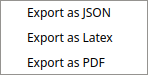
\includegraphics[width=4cm,frame]{figures/export_options.png}
  %\caption{Data Sources Overview}
\end{figure}

\begin{itemize}
  \item \nameref{sec:report_export_json}: Export to a JSON file with additional linked resources
  \item \nameref{sec:report_export_latex}: Export to a Latex file with additional linked resources
  \item \nameref{sec:report_export_pdf}: Export to a PDF file
\end{itemize} 
\  \\

\subsubsection{Export as JSON}
\label{sec:report_export_json}

This export will generate a JSON file and a list of exported resources which are linked in the JSON file. \\

The following dialog will open.

\begin{figure}[H]
    \hspace*{-2.5cm}
    \center
    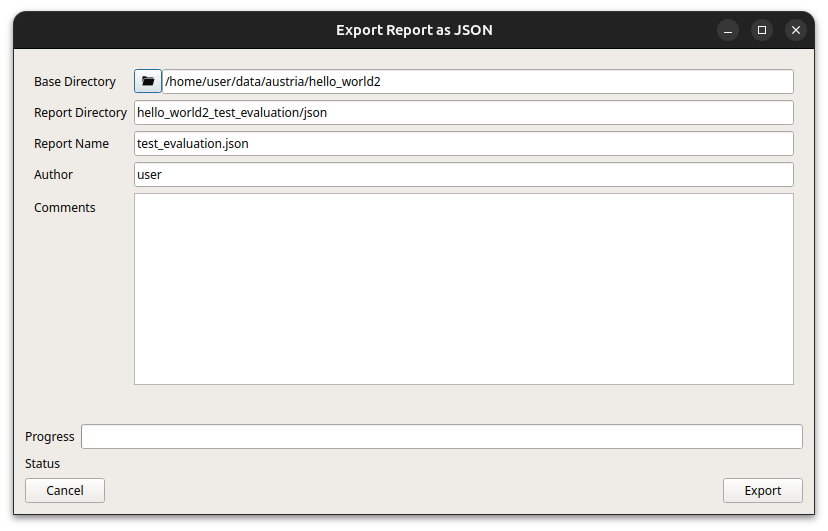
\includegraphics[width=14cm]{figures/export_json.png}
  \caption{Export as JSON}
\end{figure}

\begin{itemize}  
    \item Base Directory: Directory the report files are exported to
    \item Report Directory: Report sub-directory created inside the specified base directory
    \item Report Name: Name of the report file created
    \item Author: Name of the report's author 
    \item Comments: Optional comments
\end{itemize}
\ \\

Please \textbf{note}: The specified report sub-directory will be created inside the specified base directory.
The content of the report directory will be completely removed in this process.
Never store important data in the specified report directory. \\

When pressing 'Export' the report will be exported using the specified settings.
If the export process was sucessful, the dialog is closed automatically. \\

After export the folder structure created will e.g. look like this.

\begin{figure}[H]
    \hspace*{-2.5cm}
    \center
    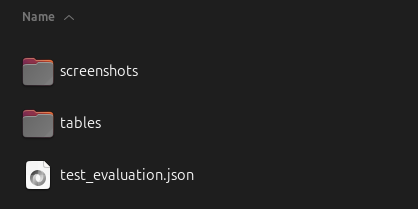
\includegraphics[width=10cm,frame]{figures/export_json_result.png}
  \caption{Export as JSON: Resulting folder structure}
\end{figure}

The folder 'tables' contains all tabular data in JSON format linked in the main JSON file.
The folder 'screenshots' contains all image data linked in the main JSON file. \\

Please \textbf{note} that all paths linked in the created JSON file are relative to the 
JSON file's directory. \\

The structure of the exported JSON is described in section \nameref{sec:report_json_struct}.

\subsubsection{Export as Latex}
\label{sec:report_export_latex}

This export will generate a Latex file and a list of exported resources which are linked in the Latex file. \\

The following dialog will open.

\begin{figure}[H]
    \hspace*{-2.5cm}
    \center
    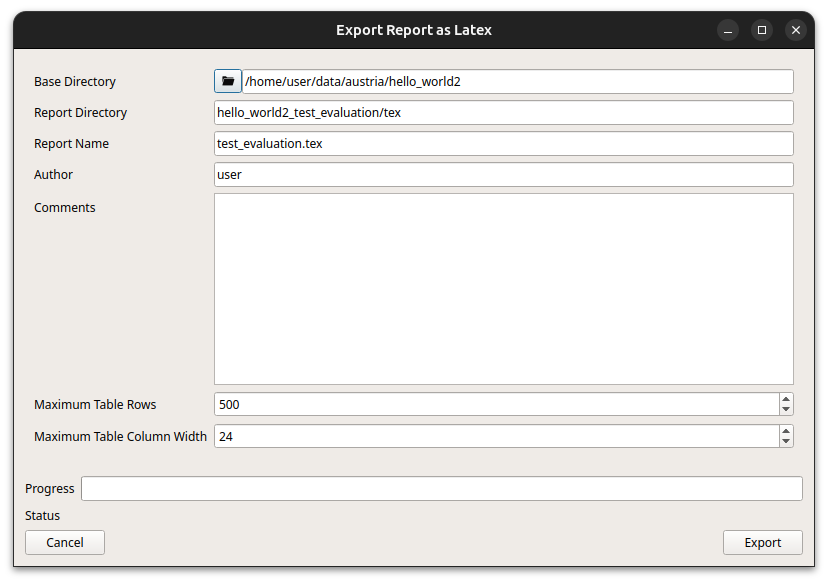
\includegraphics[width=14cm]{figures/export_latex.png}
  \caption{Export as Latex}
\end{figure}

In addition to the input fields described in Section \nameref{sec:report_export_json}, 
the following fields are available.

\begin{itemize}  
    \item Maximum Table Rows: Maximum number of rows exported to Latex tables
    \item Maximum Table Column Width: Can be used to limit Latex table column widths
\end{itemize}
\ \\

Please \textbf{note}: The specified report sub-directory will be created inside the specified base directory.
The content of the report directory will be completely removed in this process.
Never store important data in the specified report directory. \\

When pressing 'Export' the report will be exported using the specified settings.
If the export process was sucessful, the dialog is closed automatically. \\

After export the folder structure created will e.g. look like this.

\begin{figure}[H]
    \hspace*{-2.5cm}
    \center
    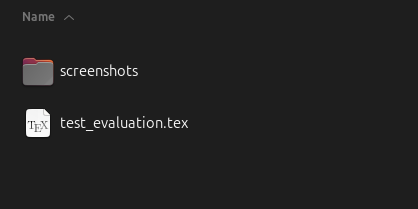
\includegraphics[width=10cm,frame]{figures/export_latex_result.png}
  \caption{Export as Latex: Resulting folder structure}
\end{figure}

\subsubsection{Export as PDF}
\label{sec:report_export_pdf}

This export will generate a PDF file. It will also create an intermediate latex file the PDF file is generated from. \\

The following dialog will open.

\begin{figure}[H]
    \hspace*{-2.5cm}
    \center
    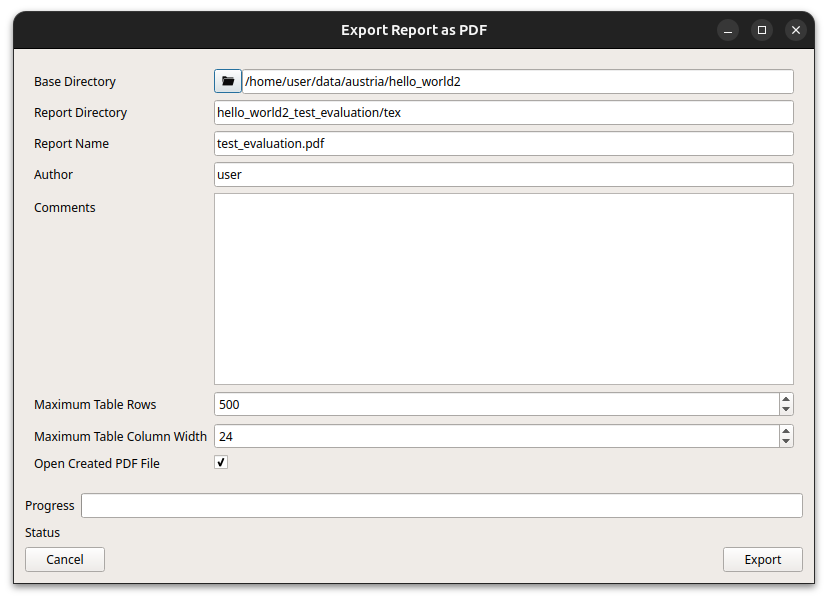
\includegraphics[width=14cm]{figures/export_pdf.png}
  \caption{Export as Latex PDF}
\end{figure}

In addition to the input fields described in Section \nameref{sec:report_export_latex}, 
the following fields are available.

\begin{itemize}  
    \item Open Created PDF File: If checked, the created PDF file will be opened in the system's default PDF viewer
\end{itemize}
\ \\

Please \textbf{note}: The specified report sub-directory will be created inside the specified base directory.
The content of the report directory will be completely removed in this process.
Never store important data in the specified report directory. \\

When pressing 'Export' the report will be exported using the specified settings.
If the export process was sucessful, the dialog is closed automatically. \\

After export the folder structure created will e.g. look like this.

\begin{figure}[H]
    \hspace*{-2.5cm}
    \center
    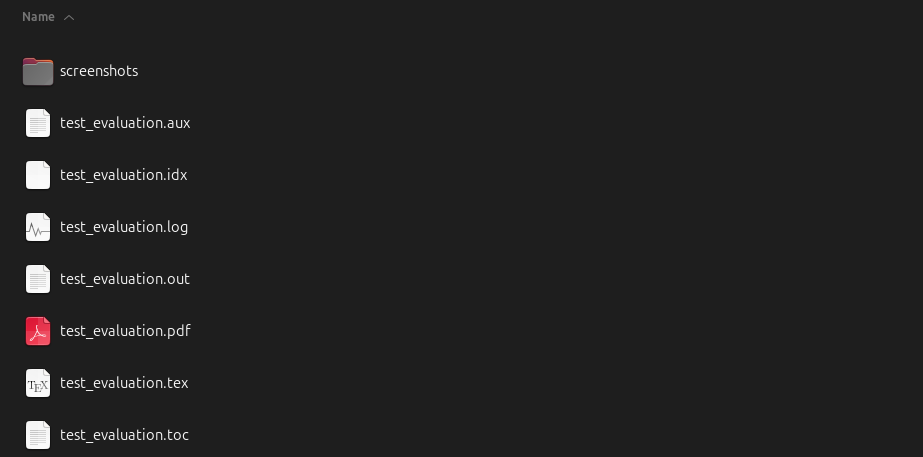
\includegraphics[width=14cm,frame]{figures/export_pdf_result.png}
  \caption{Export as PDF: Resulting folder structure}
\end{figure}

Please \textbf{note} that the generated report can of course be edited by the user and re-generated using pdflatex, 
which allows for better customization options (adding e.g. details, corporate identity etc.).

\subsection{Report Structure}

A report consists of a hierarchy of nested sections. 
A section obtains a name, and may contain multiple subsections and a number of so-called \textit{contents}.
When selecting a report in the report selection, the report's main section will be shown. \\

Above the displayed section, a couple of navigation elements reside.

\begin{figure}[H]
    \hspace*{-2.5cm}
    \center
    
\includegraphics[width=12cm,frame]{figures/navigation.png}
  \caption{Navigating sections}
\end{figure}

By pressing the \includegraphics[width=0.5cm,frame]{../../data/icons/arrow_to_left.png} button,
one can navigate back to the last displayed section.

Next to the back button the path of the currently display section in the report will be displayed.

On the right side the 'Sections' button resides. Pressing the 'Sections' button will open a table of 
contents listing all available sections.

\begin{figure}[H]
    \hspace*{-2.5cm}
    \center
    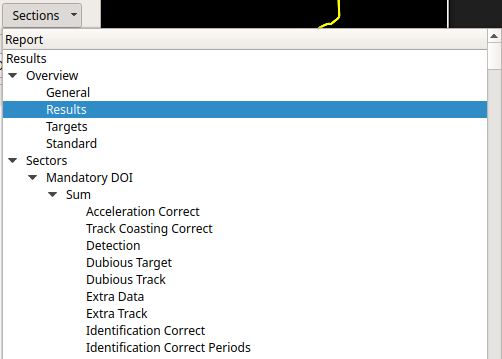
\includegraphics[width=12cm,frame]{figures/section_button.png}
  \caption{Section table of contents}
\end{figure}

Clicking a section entry once will navigate to the selected section. Double-clicking the section entry will 
in addition close the table of contents. Pressing the 'Sections' button again will close the table of contents
without selecting a section. \\

When navigating to a section, the section's contents will be displayed. \\

A section can obtain three types of contents:

\begin{itemize}  
    \item \nameref{sec:report_section_figures}: Viewable data, which can be visualized in certain Views and exported to a file as image data
    \item \nameref{sec:report_section_tables}: Tabular data, which can be inspected and exported
    \item \nameref{sec:report_section_texts}: Textual data
\end{itemize}
\ \\

\subsubsection{Figures} 
\label{sec:report_section_figures}

\begin{figure}[H]
    \hspace*{-2.5cm}
    \center
    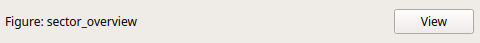
\includegraphics[width=12cm,frame]{figures/content_figure.png}
  \caption{Figure content}
\end{figure}

Figures will be displayed as a text label showing the figure's name, and a 'View' button. When pressed, the figures 
drawable contents will be shown in all Views that are able to display it.

\subsubsection{Tables} 
\label{sec:report_section_tables}

\begin{figure}[H]
    \hspace*{-2.5cm}
    \center
    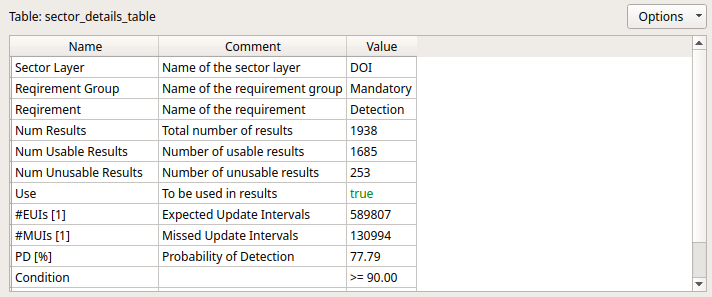
\includegraphics[width=12cm,frame]{figures/content_table.png}
  \caption{Table content}
\end{figure}

Tables will be displayed as a text label showing the table's name, the table's contents, 
and an 'Options' button. \\

Clicking the 'Options' button will show a menu.
The 'Copy Content' action can be used to copy the table's contents to the clipboard as CSV representation. \\

Table rows might additionally be linked to either viewable data or another section.
Clicking on a table row will trigger the linked viewable data to be displayed if available.
Double-clicking on a table row will navigate to the linked section if available.

\subsubsection{Texts} 
\label{sec:report_section_texts}

Texts contain textual data, which will be displayed as a list of text labels. \\

\subsection{Report JSON Structure}
\label{sec:report_json_struct}

The exported report JSON file contains the following structure. Sections are exported as follows.

\begin{lstlisting}[basicstyle=\small\ttfamily]
{
    "contents": [ SECTION_CONTENTS ],         // List of section contents
    "name": "Results",                        // Section name
    "sub_sections": [ NESTED_SUB_SECTIONS ]   // List of nested sub-sections
}
\end{lstlisting}

Contents are exported as follows.

\begin{lstlisting}[basicstyle=\small\ttfamily]
{
    "content_type": CONTENT_TYPE,            // Content type: "table"/"figure"/"text"
    "name": "gen_overview_table",            // Content name 
    
    ...                                      // Additional content-specific fields
}
\end{lstlisting}

Specific contents will in addition obtain special fields storing their data.

\paragraph{Tables} Tables can contain the following attributes in addition.

\begin{itemize}  
  \item columns: List of strings describing the table's columns
  \item data: List of lists containing the table's individual columns
  \item path: Relative path to an external json file containing a JSON object with the table data fields "columns" and "data"
\end{itemize}

\paragraph{Figures} Figures can contain the following attributes in addition.

\begin{itemize}  
  \item data\_base64: base64-encoded PNG image data stored as a string
  \item path: Relative path to an external image file
\end{itemize}

\paragraph{Texts} Texts can contain the following attributes in addition.

\begin{itemize}  
  \item texts: List of text strings
\end{itemize}
